\documentclass[10pt]{ujarticle}
\usepackage{float}
\usepackage{adrobo_abst}
\usepackage{graphicx}
\usepackage[dvipdfmx]{color}
\usepackage{amssymb,amsmath}
\usepackage{bm}
\usepackage[superscript]{cite}
\usepackage{enumerate}
\usepackage{url}
% \usepackage[dvipdfmx]{color}
%\usepackage[absolute]{textpos}

\renewcommand\citeform[1]{(#1)}

\begin{document}
    
    \makeatletter
    \doctype{2022年度卒業論文概要}
    \title{視覚と行動のend-to-end学習により経路追従行動をオンラインで模倣する手法の提案}{(オフラインでデータセットを収集して訓練する手法の提案)}
    \etitle{A proposal for an online imitation method of path-tracking
    behavior by end-to-end learning of vision and action}{(Validation of a method to collect and train dataset offline)}
    
    \author{19C1068\hspace{.5zw}髙橋祐樹}
    \eauthor{Yuuki TAKAHASHI}
    
    \makeatother
    
    \abstract{In this paper, we propose a method to collect and train data offline, based on the conventional method to mimic path-following behavior. Experimental results show the effectiveness of the proposed method. }
    
    \keywords{End-to-End Learning, Navigation, Offline}
    
    \maketitle
    
    \supervisor{指導教員:林原靖男 教授}
    
    \section{緒\hspace{2zw}言}%===========================
    近年, 自律移動ロボットの研究が盛んに行われている. Bojarskiら\cite{bojarski}は人が操作するステアリングの角度をend-to-end学習することで, 自律走行する手法を提案した. また, 岡田ら\cite{si2020-okada}\cite{si2021-okada}(以下「従来研究」と称する)により2D-LiDARを用いた自律移動システムの出力をロボットに与えて学習させることで, 経路追従行動をオンラインで模倣する手法を提案し, 実験によりその有効性を確認してきた. しかし, カメラ画像を入力とした学習器の出力のみで自律走行をするためには, ロボットを何周も走行させて学習する必要がある. これでは, 走行中にロボットがコースアウトしないか監視する必要や, 時間がかかるといった問題点がある. そこで, 本研究では, 従来手法を基に, 目標とする経路上及び周辺のデータを一度に収集し, オフラインで訓練する手法を提案する. 提案手法では, 経路上にロボットを配置し, カメラ画像と教師データとなる目標角速度を収集する. それらのデータを基にオフラインで学習を行い, 学習後はカメラ画像を入力とした学習出力により自律移動させることで, 手法の有効性を検証する. 
    % また, 清岡ら\cite{si2021-kiyooka}により, 経路上だけでなく経路から離れた状態も学習することが, 経路追従行動を模倣する上で有効であることも示されている.

    \begin{figure}[!b]
        \centering
        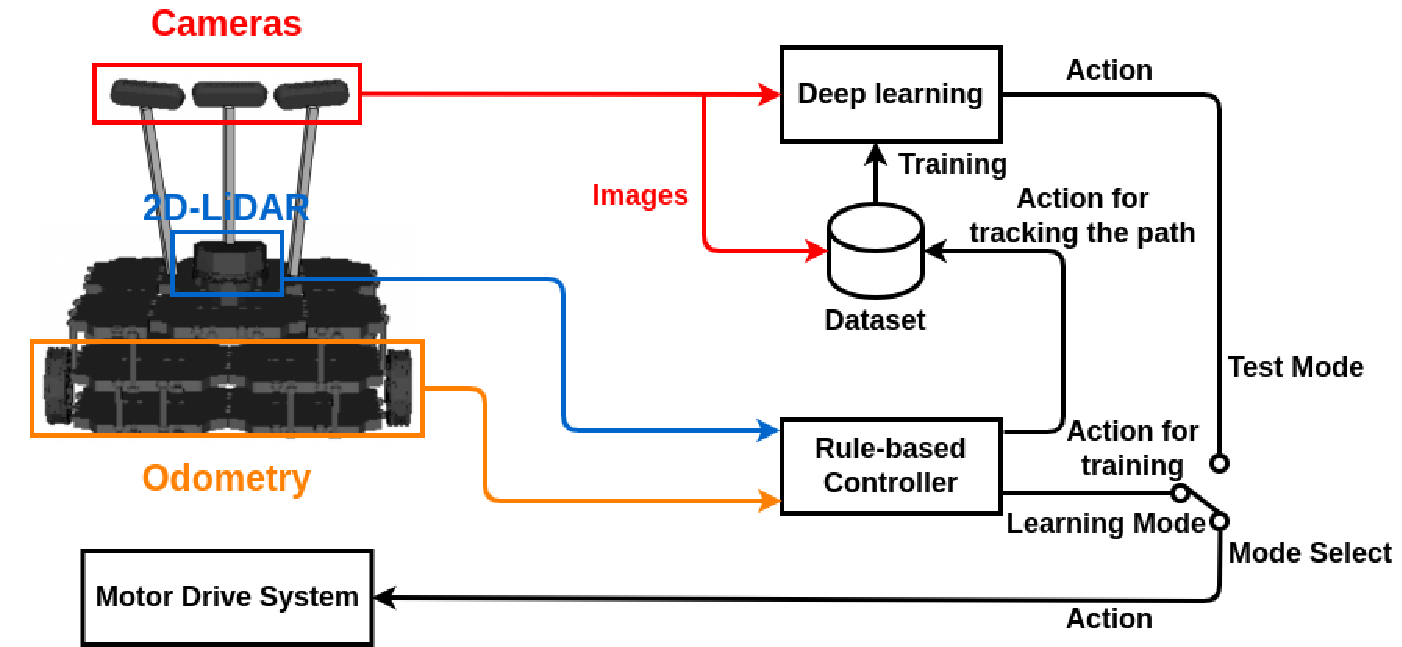
\includegraphics[width=0.5\textwidth]{fig/okada.pdf}
        \caption{Systems that imitation learning for map-based navigation from\cite{si2020-okada}}
        \label{Fig:si2020-okada}
    \end{figure}
    
    \section{従来手法}%===========================
    従来研究の概要を以下で述べる. 従来研究では, 地図を用いたルールベース制御器によるナビゲーションの走行を模倣し, 視覚に基づく経路追従行動を獲得した. 従来研究のシステム概要を図\ref{Fig:si2020-okada}に示す. システムでは, LiDAR, オドメトリを入力としたナビゲーションの出力である角速度を学習器とモータ駆動系に与える. ナビゲーションの角速度は, ROSのパッケージであるnavigation\cite{navigation}により計算される. また, 学習器には, カメラ画像を64×48にリサイズした3つのカメラ画像を入力し, ナビゲーションの角速度を出力して, 0.2[s]の周期でend-to-end学習する. 左右のカメラ画像に対する目標角速度には, それぞれ経路に戻るようなオフセットを加える. 学習には, 入力層1, 畳み込み層3, 全結合層2, 出力層1の計7層で構成されたネットワークを用いる. 学習後は, カメラ画像のみを入力とした学習器の出力により走行する. 

    \section{提案手法}%===========================
    次に, 従来研究を基にしたオフラインでデータを収集し訓練するする手法を提案する. 図\ref{Fig:collect}にデータの収集方法を示す. 赤色の線である目標経路から平行に離れた座標にロボットを配置する. そして, その座標ごとに目標経路に沿った向きを基準として±5度傾けて, 64×48のカメラ画像(RGB画像)とルールベース制御器によるナビゲーションの出力である角速度をのように収集する. ただし, ロボットの進行方向に対する並進速度は0[m/s]であるが, データセットにはナビゲーションの出力である角速度がロボットに与えられる. このように, ロボットを走行させることなく, 目標経路上及び周辺に配置することで, 一度に大量のデータを収集することができる. その後, 収集したデータを使用してオフラインで学習を行う. 

    \begin{figure}[h]
        \centering
        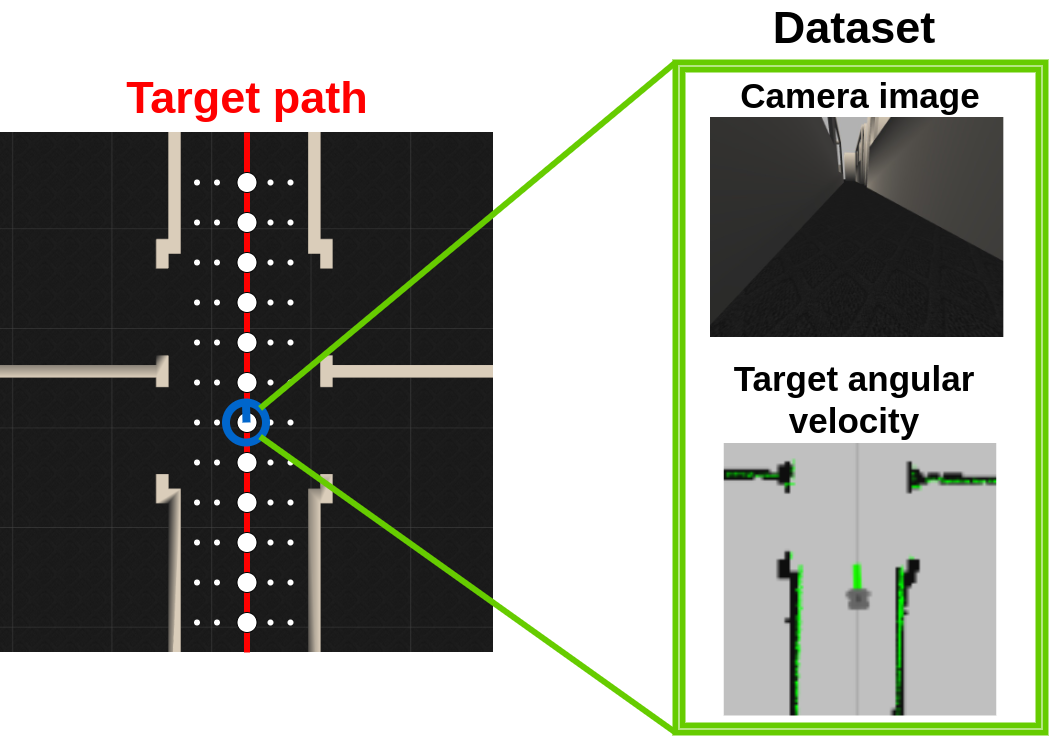
\includegraphics[width=0.4\textwidth]{fig/collect-data2.png}
        \caption{Method of collecting data around the target route}
        \label{Fig:collect}
    \end{figure}

    \section{シミュレータを用いた実験}%===========================
    \subsection{実験目的}\mbox{}\\
    シミュレータ上で実験を行い, 提案手法の有効性を検証する. 

    \subsection{実験装置}\mbox{}\\
    シミュレータにはGazebo\cite{gazebo}のWillow Garage{willow}でに示すコーで一周行う. また, ロボットモデルにはカメラを3つ搭載したTurtlebo3\cite{turtlebot3}を用いた. 

    \subsection{実験方法}
    \begin{enumerate}
        \item{データ収集フェーズ}\mbox{}\\データの収集方法について述べる. 図\ref{Fig:collect-data}にデータの収集方法を示す. 赤色の線である目標経路から平行に平行に±0.01, ±0.02, ±0.04, ±0.06, ±0.08, ±0.10, ±0.15, ±0.20, ±0.30[m]離れた座標にロボットを配置する. そして, その座標ごとに目標経路に沿った向きを基準として±5度傾けて, カメラ画像とナビゲーションの出力である角速度を収集する. これをに示したコースで一周行う. 
        \item{訓練フェーズ}\mbox{}\\従来研究ではオンラインで学習を行うため計算のリソースなどの観点からバッチサイズを8にして, 全てのデータを使用していなかった. しかし, 本研究ではオフラインで学習を行う特徴を活かして, 全てのデータを使用するバッチ学習を用いる. データ量及びバッチサイズ7242, 4000step, 8000step, 10000step学習した. なお, 4000stepは従来研究において, シミュレータの実験に用いられてきたステップ数であり, 10000stepは従来研究において, 実ロボットの実験に用いられていたステップ数である. 
        \item{テストフェーズ}\mbox{}\\に示したコースで10回走行させる. 壁に衝突せずに一周できた場合を成功とし, 壁に衝突したり, コースアウトして経路に復帰できなかったりした場合を失敗とした. 
    \end{enumerate}

    \begin{figure}[h]
        \centering
        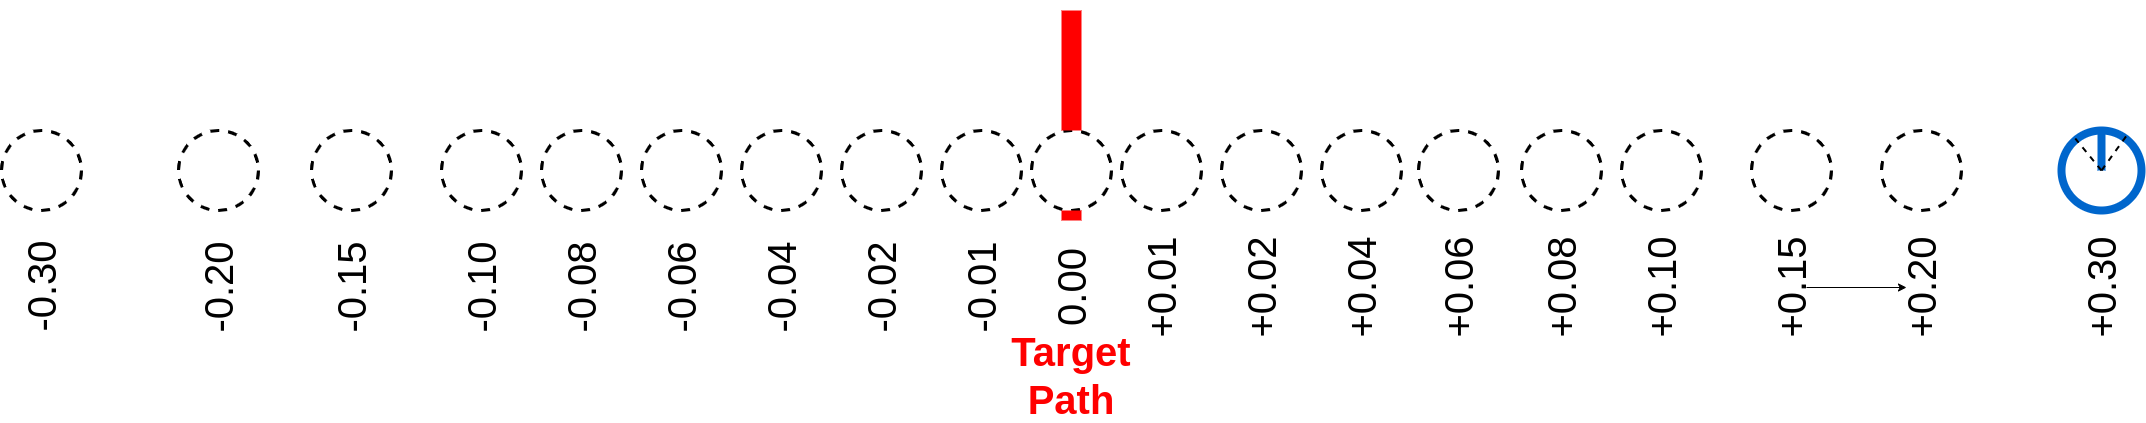
\includegraphics[width=0.45\textwidth]{fig/collect-data.png}
        \caption{Method of collecting data around the target route}
        \label{Fig:collect-data}
    \end{figure}

    \subsection{実験結果}\mbox{}\\
    実験結果を表\ref{tb:result}, lossのグラフをに示す. 4000stepでは成功回数が0/10だったが, 8000step, 10000stepにすることで成功回数が1/10になり, 目標経路を一周することができた. また, からステップ数増やすことで学習が収束していることが確認できる. このことから, 訓練する際にバッチ学習を用いて, ステップ数を増やすことで成功回数が増えることを示せた. 

    \begin{table}[h]
        \centering
        \begin{tabular}{|c|c|} \hline
          Experiments & Number of successes \\ \hline
          Exp.1(4000step) & 0/10 \\ \hline
          Exp.2(8000step) & 1/10 \\ \hline
          Exp.3(10000step) & 1/10 \\ \hline
        \end{tabular}
        \caption{Number of successes in the experiment}
        \label{tb:result}
      \end{table}

    \section{結\hspace{2zw}言}%===========================
    本稿では, 従来から提案する経路追従行動を模倣する手法を基に, オフラインでデータセットを収集して訓練する手法を提案した. そして, 実験により提案手法の有効性を確認した. 

    \vspace{5truemm}
    {\footnotesize
        \begin{thebibliography}{99}

            \bibitem{bojarski}
            Bojarsi, Mariusz, et al.:``End to End Learning for Self-Driving Cars.'', arXiv: 1604.07316, 2016
            
            \bibitem{si2020-okada}
            岡田 眞也, 清岡 優祐, 上田 隆一, 林原 靖男: ``視覚と行動のend-to-end学習により経路追従行動をオンラインで模倣する手法の提案'', \textit{計測自動制御学会 SI 部門講演会 SICE-SI2021 予稿集}, pp.1147-1152, 2020.

            \bibitem{si2021-okada}
            岡田 眞也, 清岡 優祐, 春山 健太, 上田 隆一, 林原 靖男: ``視覚と行動のend-to-end学習により経路追従行動をオンラインで模倣する手法の提案-“経路追従行動の修正のためにデータセットを動的に追加する手法の検討'', \textit{計測自動制御学会 SI 部門講演会 SICE-SI2021 予稿集}, pp.1066-1070, 2021.

            \bibitem{si2021-kiyooka}
            清岡 優祐, 岡田 眞也, 岩井 一輝, 上田 隆一, 林原 靖男: ``視覚と行動のend-to-end学習により経路追従行動をオンラインで模倣する手法の提案''-データセットと生成された経路追従行動の解析'', \textit{計測自動制御学会 SI 部門講演会 SICE-SI2021 予稿集}, pp.1072-1075, 2021.

            \bibitem{navigation}
            ros-planning, navigation リポジトリ\\
            \url{https://github.com/ros-planning/navigation}\\
            (最終閲覧日 \today)

            \bibitem{gazebo}
            gazebo リポジトリ\\
            \url{http://gazebosim.org/}\\
            (最終閲覧日 \today)

            \bibitem{willow}
            Koenig, Nathan, and Andrew Howard. ”design and use paradigms for gazebo, an open-source multi-robot simulator.”. 2004 IEEE/RSJ International Conference on Intelligent Robots and Systems (IROS)(IEEE Cat. No. 04CH37566). Vol. 3. IEEE, pp.2149-2154(2004).\\
            (最終閲覧日 \today)

            \bibitem{turtlebot3}
            Turtlebot3-obotis emanual.robotis.\\
            url{https://emanual.robotis.com/docs/.}\\
            (最終閲覧日 \today)
            
        \end{thebibliography}
    }
\end{document}
